%   Filename    : chapter_4.tex 
\chapter{Research Methodology}
This chapter presents the tools, techniques, and methodologies that was used for the development of TUKIB. This chapter also specifies the software and hardware requirements, as well as, the comprehensive processes included in creating the system.

\section{Research Activities}

\subsection{Development Framework}

\textbf{Agile Methodology}

\noindent The software development approach that the developers followed in developing TUKIB is the agile methodology. Agile methodology, or simply agile, is a framework that emphasizes iterative development and features communication and collaboration, adaptive planning, and continuous development (Agile Framework, 2022). The developers chose this framework because of its flexibility and adaptability to change, which is beneficial, especially with evolving user requirements. 

As seen from \figref{fig:agile}, agile involves continuously cycling through phases of development, testing, and review or feedback before finally launching the system. This enables developers to make adjustments and improvements based on user input. \newline

\begin{figure}[h]
	\centering 
	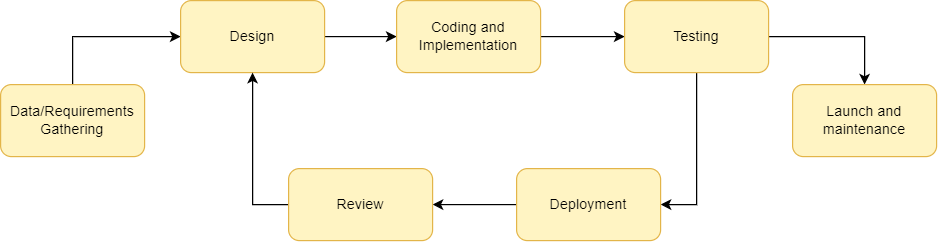
\includegraphics[width=1\textwidth]{agile methodology.png}
	\caption{Agile Methodology}
	\label{fig:agile}
\end{figure}

\noindent\textbf{Data Gathering and Documentation}
	
\noindent The developers began the project by visiting the UPV RRC, where they conducted interviews with stakeholders. This phase was essential for gaining a comprehensive understanding of the institution's specific needs and for planning the system features accordingly. The data gathered during these interviews guided the subsequent phases of the project, ensuring that the system is tailored to meet the requirements and expectations of its users. 

This phase includes the following activities:

\begin{itemize}
	\item \textbf{Defining Objectives.} Establishing the primary goals of TUKIB based on preliminary research and stakeholder input, ensuring that the project aligns with user needs.
	\item \textbf{Stakeholder Identification.} Identifying key stakeholders, including RRC personnel and potential users, to ensure that a diverse range of needs is considered and addressed throughout the development process.
	\item \textbf{Defining User Requirements.} Collecting and analyzing user requirements through interviews and interactions with stakeholders. This will involve creating user stories to capture the specific needs and expectations of different user groups, ensuring that the system design is informed based on real-world usage scenarios.
\end{itemize}
	
\noindent\textbf{System Design}
	
\noindent After data gathering, the system's architectural design was developed. This process involved creating a context model to outline the system's interactions with external entities, as well as a data flow diagram to illustrate how data moves through the components of the system. A process flow diagram was also constructed to detail the specific processes and workflows, while database models will be designed to ensure efficient data storage and retrieval. 

The researchers also focused on effective user interfaces (UI) for service request handling and management, investigating best practices and design principles that enhance user experience based on feedback from users of existing similar software or systems. Once all necessary information is gathered, a mock-up design of TUKIB was created, serving as the basis for the system's prototype. Together, these diagrams and designs provided a comprehensive framework that will guide the development and implementation of the system effectively.\newline
	
\noindent\textbf{Implementation}
	
\noindent From the design phase, the development of the system started. The frontend was built with the intention to ensure a user-friendly interface while the backend supports functionality through efficient data processing and secure user authentication. A chatbot was also integrated to facilitate real-time client support and interaction with the system.

Since the developers are following the Agile methodology, the implementation phase occured alongside testing. This iterative process involved cycles of development and testing during each sprint, with each sprint lasting two weeks. This approach allowed for continuous feedback and improvements, ensuring further that the system meets user needs effectively.\newline
	
\noindent\textbf{Testing}

\noindent The testing of the system was be consisted of 3 main components to ensure its reliability, usability, and overall performance.

\begin{itemize}
	\item \textbf{Alpha Testing.} During and after the development of each feature, extensive user testing was conducted to ensure that each feature works as intended. Any bugs or problems was immediately fixed. For features dependent on other features (i.e. user account creation must function correctly before user can log in), thorough testing ensured and verified that the integration between these features operates smoothly.
	
	\item \textbf{Automated testing.} Automated testing was implemented to ensure reliability and efficiency in testing the features of the system. This approach allowed for the execution of predefined test cases that can be run repeatedly with minimal manual intervention.
	
	\item \textbf{Beta Testing.}  Beta testing was be done with a limited group of users composed of available RRC staff and selected potential customers of RRC (e.g. students and faculty). This phase allowed real-world usage feedback and helped in identifying any remaining bugs and usability issues. Users tested the system in various environments and encouraged to provide insights on functionality, performance, and overall experience.\newline
\end{itemize}
	
\noindent\textbf{Deployment and Maintenance}

\noindent The final product of the study, TUKIB, will made available to the intended users. In this phase, ongoing maintenance and regular performance monitoring, especially of the backend, are essential to ensure stability and reliability. Feedback form will be issued to users in to gather their thoughts and insights about the system or if they have encountered any bugs. Constant feedback from users during this phase will guide further improvements and updates.

\section{Chatbot architecture and development}

This section outlines the architecture of the Rasa framework, as well as, the necessary information on how the chatbot will be developed.

\subsection{Rasa Chatbot Architecture}

The chatbot for the system was created using the Rasa framework. Rasa is an open source conversational AI framework that allows developers to build, deploy, and improve AI-powered chatbots and virtual assistants. \figref{fig:rasa_architecture} shows the details about the architecture of Rasa chatbot design. Specifically, this study utilized the Open Source framework of Rasa.

There are two main components in Rasa Open Source architecture namely: Rasa NLU and Rasa Dialogue Policies. The Rasa NLU, shown as NLU pipeline in the figure, is like the primary senses of the chatbot which receive the input from the users. It identifies, classifies, and extracts the intents and entities from the given input. It is also responsible for choosing and retrieving the appropriate response to the user. 

The dialogue management also called the Rasa Core, shown as Dialogue Policies in the figure, decides the next action in a conversation based on the context of the conversation. Rasa SDK is an action server which is responsible for running custom actions. The Tracker store is where the conversations are stored. The chatbot saves the context which helps give personalized interactions with the user as it learns over time. Rasa also uses a ticket lock mechanism to ensure that incoming messages for a given conversation ID are processed in the right order, and locks conversations while messages are actively processed. This allows for multiple Rasa servers to be run in parallel. File system consists of Models and Training data needed for the functionality of the chatbot.

\begin{figure}[h]
	\centering 
	\includegraphics[width=1\textwidth]{RASA_architecture.png}
	\caption{Rasa Open Source Chatbot Architecture}
	photo from https://rasa.com/docs/rasa/arch-overview/
	\label{fig:rasa_architecture}
\end{figure}

\subsection {Conversation Processing}

Rasa mainly includes three stages in its conversation processing. They are:

\begin{itemize}
	\item \textbf{NLP pipeline (Natural Language Processing)}
	
	The input or message is given by the user in this stage. The chatbot mainly tries to understand the context of the user’s message and meaningful information is extracted. This stage involves tokenization, intent and entity recognition, and featurization. The extracted information is then mapped or matched with the training data.
	
	\item \textbf{Dialogue management (Response selection stage)}
	
	Once the input is processed by the NLP pipeline, it proceeds to the dialogue management stage. This stage involves decision-making about how the bot should respond based on the user’s given input and the context of the conversation. 
	
	\item \textbf{Response Generation / Output}
	
	Once the appropriate response or action has been determined, the final stage is to generate the bot’s response to the user.  There are two main approaches for generating these responses. First is the template-based responses which are the pre-defined response templates based on the extracted intent and entities from the user’s message. These responses are static and are typically used for simple and predictable replies. Another is the custom action. This is for complex responses, such as calling an API or performing specific logic. For example, the chatbot will call from the backend to fetch service details or event schedules, and then dynamically generate a response based on the result.
	
\end{itemize}


\subsection{Model Training}

For this study, the training data used was in the form of conversations between the RRC staff and clients during previous consultations. The data collection was done with the help of RRC staff to ensure its accuracy and validity. The gathered data was used to train Rasa’s NLU model, allowing it to recognize user intents and extract relevant information accurately. As per Rasa’s capability, continuous use of the chatbot further trains the model, allowing it to learn from interactions and improve its understanding over time. This ongoing training process will enhance the chatbot’s performance, ensuring it becomes more adept at addressing user needs and providing relevant and more accurate responses as it accumulates more data from real-world users.

\subsection {Limitations of Rasa}

Rasa is a powerful open-source framework for building conversational AI applications, but like any other technology implemented, it also has its limitations. The first is that Rasa has a higher learning curve. To be able to use Rasa, developers must know Python, machine learning concepts, and experience in natural language processing. Without these Rasa wont be set up and utilized effectively. 

Another is how Rasa is highly dependent on training data. In another view, this may help the developers customize the responses and conversations to their specific needs. However, when training is poorly done and insufficient data is given, this results in low chatbot accuracy. This backfires and counters the purpose of chatbots in providing accurate assistance. Hence, extensive training data to account for various scenarios and user inputs is needed for proper context modeling.

\section{Storage and Database Architecture}

This section outlines how data is stored and the strategies that was used for the efficiency and scalability of the database of TUKIB, ensuring that the system can handle growing amounts of service requests, data, and users over time without compromising its performance or reliability.

\subsection{Storage and Archiving}

TUKIB utilizes PostgreSQL as its database, organizing data into two separate databases to make management easier. One database stores active data, like recent service requests and client interactions, while the other is used for archived data. By separating active and archived data, the RRC can keep the active database fast and responsive while still being able to access older data when needed.

To manage data growth, records or data older than a year will automatically be moved into the second database. This is done through scheduled scripts, freeing up space in the active database and ensuring that the system runs efficiently.

\subsection{Distributed and Scalable Database Architecture}

To support the growth of the system, horizontal scaling strategy was implemented to manage increased traffic and larger volumes of data. PostgreSQL offers built-in functionality to set up read replicas, which will be used to distribute query loads and improve response times, especially for read-heavy operations such as retrieving recent service requests.

When necessary, data partitioning (sharding) can be applied to the archived database to split the large datasets across multiple servers. This approach will ensure better performance and scalability as the volume of archived data continues to grow.

Additionally, regular automated backups will be scheduled for both the active and archived databases using PostgreSQL's built-in backup functions. These backups will ensure data durability and enable quick recovery in case of failures, avoiding disruptions in RRC’s service delivery.
 
\section{Development Tools}

\subsection{Hardware}

The hardware requirements for the development of the system include a computer or laptop with the following specifications:

\begin{itemize}
	\item Processor: Intel Core i5, its equivalent on other brands or higher
	\item RAM: 6GB or higher
	\item Storage: 200GB SSD or more for faster data access and retrieval
	Operating System: Windows 10 or higher, macOS, or Linux
\end{itemize}

These specifications are necessary to ensure smooth development and testing of the system, especially when handling large datasets and concurrent processes.

\subsection{Software}

TUKIB will be developed using a range of modern software tools tailored to meet the specific needs of the research center’s workflow automation and data management processes.

\begin{itemize}
	\item \textbf{HTML5, CSS, Bootstrap, and ReactJS}
	
	These technologies will be used for front-end development of the system. HTML5 will structure the webpages, CSS will be responsible for the visual styling, Booststrap for UI $ $flexibility, and ReactJS enables dynamic and interactive user interfaces.\newline
	
	\item \textbf{PostgreSQL}
	
	For backend development, PostgreSQL is will be used as the database management system, offering robust data storage, querying, and management capabilities.\newline
	
	\item \textbf{Rasa Framework}
	
	Rasa will be used for the chatbot development. It allows the creation of a conversational AI system which will handle the service requests, queries, and management capabilities of the system.\newline
	
	\item \textbf{Figma}
	
	Figma will be utilized for designing the UI/UX of the system. Figma allows design collaboration, which will ebavle the team to create the system prototype, wireframe, and mock-up interfaces before implementation, ensuring a user-friendly experience for both clients and researchers.\newline
	
	\item \textbf{VS Code}
	
	Visual Studio Code (VS Code) is the primary code editor that will be used to develop the system. Its features, such as syntax highlighting, extensions, integrated Git, and debugging tools, make it the most suitable environment for writing and testing front-end and back-end code.\newline
	
	\item \textbf{Github}
	
	GitHub will be used to facilitate for version control and collaboration thoughout the development of the system. The project code is stored in repositories, allowing the team to manage changes, track progress, and collaborate effectively. It also serves as a backup and source for future development or modification.
	
\end{itemize}


